% 5. Einleitung

\chapter{Results and Discussion}

When applying all corrections, presented in chapter~\ref{chap:fvz}, to the measured zenith angles $z_b$ one obtains the true zenith angles $z$ as presented in Fig.~\ref{fig:zenith}. The zenit angles are given as a function of universal time (UT) in hours, at which the individual measurements have been taken. 
From the decreasing value of $z$ with time, one can deduce that all measurements have been taken before noon, since a rising sun coencides with decreasing zenith angles. \\ The error bars in Fig.~\ref{fig:zenith} correspond to the error of the zenith angle $z$ and are, in this representation, barely visible. The fact that some of the data points deviate significantly from the expected errors can be attributed to the fact that the central crosshair in the theodolite's scope was reported to be mistaken with one of the outer crosshairs for some of the measurements. Additional contributions to the error might come from the fact that the theodolite is not perfectly leveled, giving an unknown error.\\


\begin{figure}[]
    \centering
    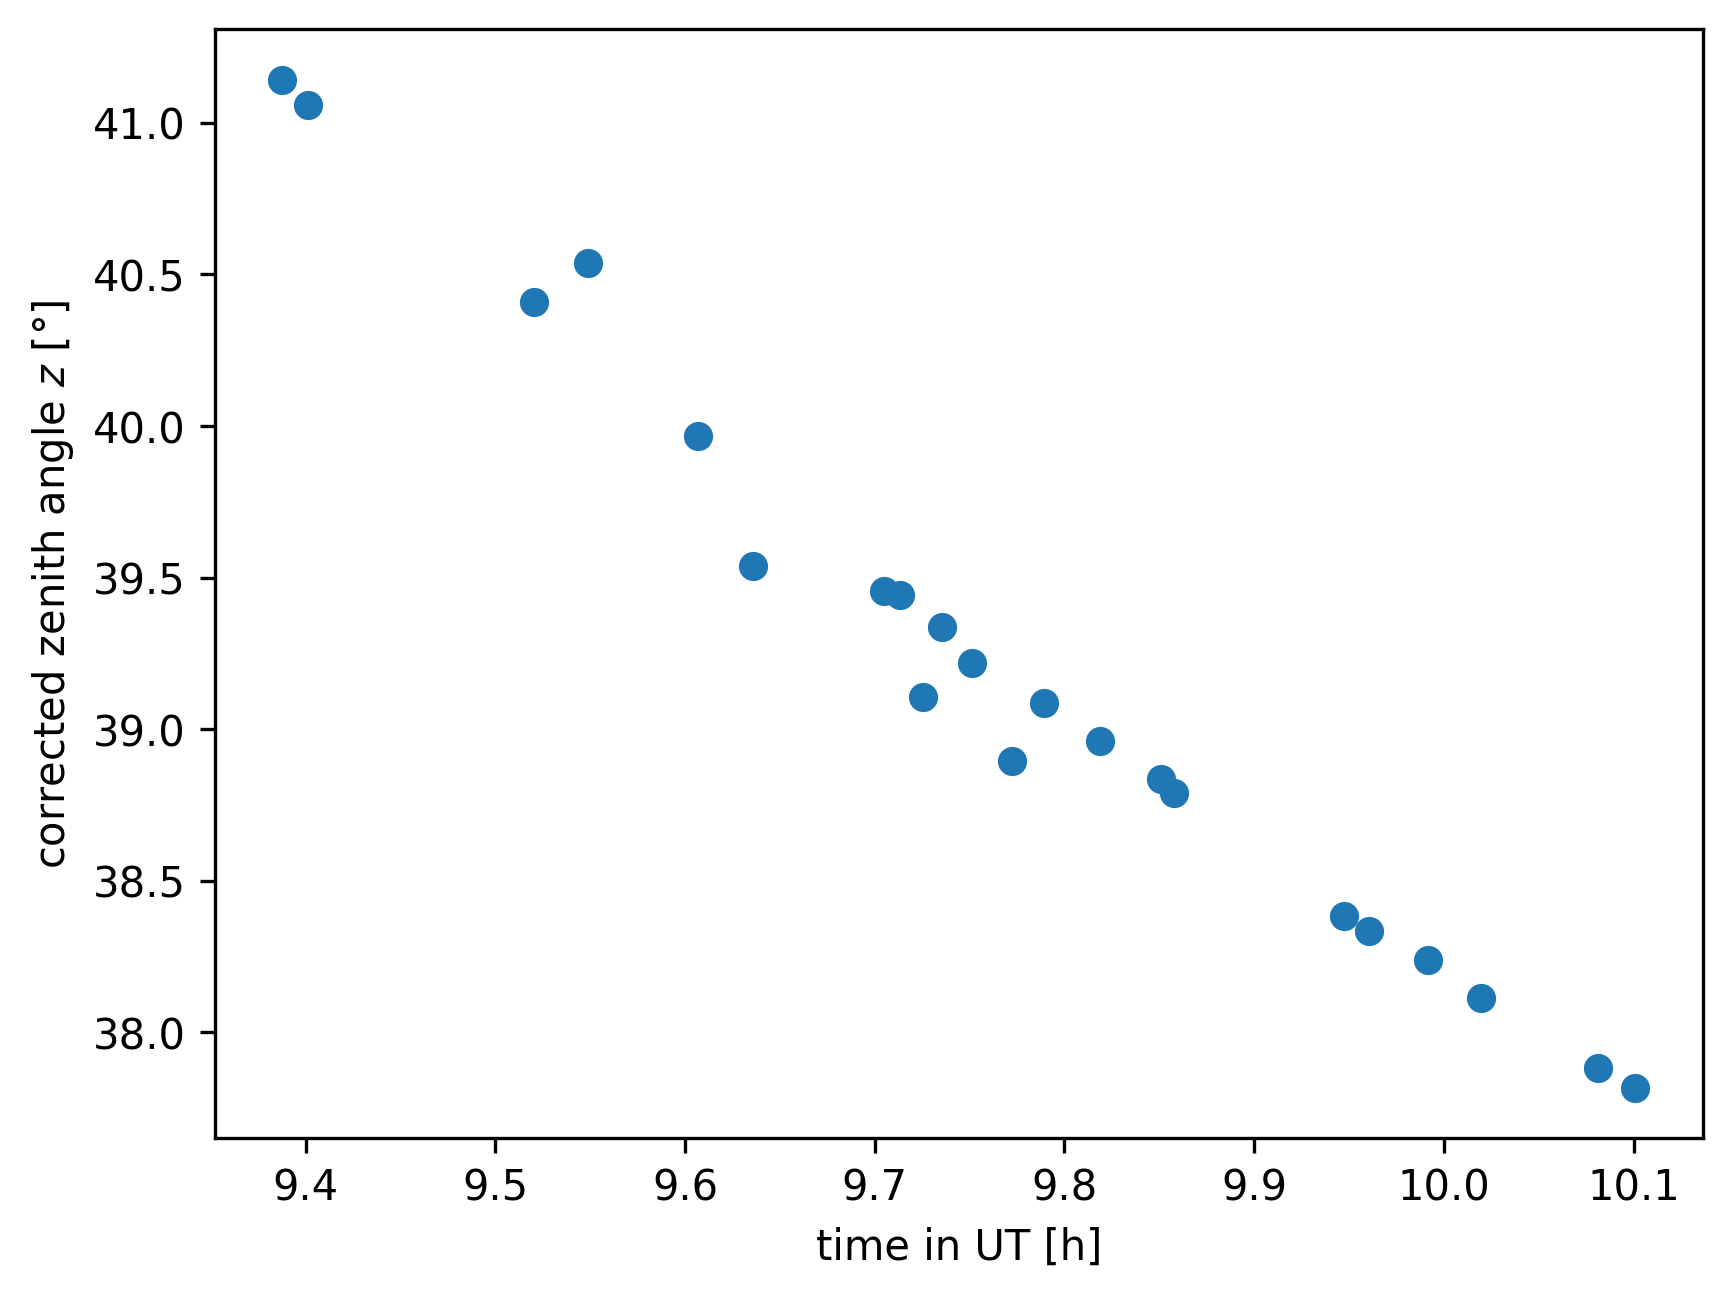
\includegraphics[width=0.9\textwidth]{05-Fazit/zenith_angle_plot.png}
    \caption{Corrected zenith angle $z$, obtained according to Eq.~(\ref{eq:zenith_angle_corrections}), as function of measurement time in UT.}
    \label{fig:zenith}
\end{figure}

\label{chap:fazit}


% Text